\subsection{Model derivation}
\label{subsec:model_derivation}

The \acrshort{mls} is a complex system that can be divided into two main subsystems:

\begin{itemize}
    \item \textbf{Electromagnetic subsystem}: it takes into account the electrical components of the system from the power supply to the generation of the magnetic field by the coils;
    \item \textbf{Mechanical subsystem}: it takes into account the dynamics of the ball and all the forces acting on it, including the electromagnetic forces generated by the electromagnetic subsystem.
\end{itemize}

Due to the presence of the ball that moves inside a magnetic field, a complex connection between the two subsystems that goes beyond the simple force balance exists.
For this reason, it's almost impossible to derive a complete model of the system without considering both subsystems at the same time.

In the following sections, we will derive the equations that governs the \acrshort{mls} system, adopting an energetic approach that takes into account the energy conservation principle.

\subsubsection{Mathematical model}
\label{subsubsec:mathematical_model}

In Figure \ref{fig:system_model}, a schematic representation of all the components of the \acrshort{mls} system is shown.

\begin{figure}[H]

    \centering

    \begin{circuitikz}
        \draw (0,0) node [right] {$+$}
        to [short] ++(0, -1)
        to [R, l^=$R_1$, resistors/zigs=6] ++(2, 0)
        to [variable cute inductor, i>^=$I_1$, l=$L_1$] ++(2, 0)
        to [short] ++(0, +1) node [right] {$-$};
    \end{circuitikz}

    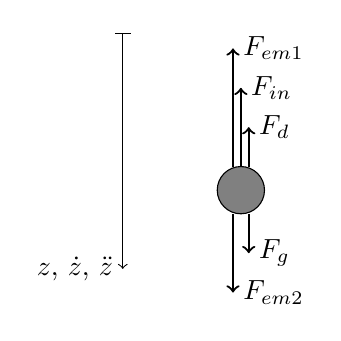
\begin{tikzpicture}

        \def\radius{0.3}

        % Reference system
        \draw[|->] (-1.5, +2.0) -- ++(0, -3) node[left] {$z$, $\dot{z}$, $\ddot{z}$};

        % Ball
        \filldraw[fill=gray, draw=black] (0, 0) circle (\radius);

        % Upward forces
        \draw[thick, ->] (-0.1, +\radius) -- ++(0, +1.5) node[right] {$F_{\text{em1}}$};
        \draw[thick, ->] (+0.0, +\radius) -- ++(0, +1.0) node[right] {$F_{\text{in}}$};
        \draw[thick, ->] (+0.1, +\radius) -- ++(0, +0.5) node[right] {$F_{\text{d}}$};

        % Downward forces
        \draw[thick, ->] (+0.1, -\radius) -- ++(0, -0.5) node[right] {$F_{\text{g}}$};
        \draw[thick, ->] (-0.1, -\radius) -- ++(0, -1.0) node[right] {$F_{\text{em2}}$};

    \end{tikzpicture}

    \begin{circuitikz}
        \draw (0,0) node [right] {$+$}
        to [short] ++(0, +1)
        to [R, l_=$R_2$, resistors/zigs=6] ++(2, 0)
        to [variable cute inductor, i>_=$I_2$, l_=$L_2$] ++(2, 0)
        to [short] ++(0, -1) node [right] {$-$};
    \end{circuitikz}

    \caption{Schematic representation of the \acrshort{mls} system.}
    \label{fig:system_model}

\end{figure}

Before proceeding with the derivation of the equations, we can give a brief description of the components of the system:

\begin{table}[H]
    \centering
    \begin{tabular}{|c|l|c|}
        \hline
        \textbf{Component} & \textbf{Description}                               & \textbf{Units} \\
        \hline
        $R_1$              & Resistance of the coil 1                           & $\Omega$       \\
        $L_1$              & Inductance of the coil 1                           & H              \\
        $I_1$              & Current flowing through the coil 1                 & A              \\
        $F_{\text{em1}}$   & Electromagnetic force generated by the coil 1      & N              \\
        $F_{\text{in}}$    & Inertial force due to the acceleration of the ball & N              \\
        $F_{\text{d}}$     & Drag force due to the air resistance               & N              \\
        $F_{\text{g}}$     & Gravitational force acting on the ball             & N              \\
        $F_{\text{em2}}$   & Electromagnetic force generated by the coil 2      & N              \\
        $R_2$              & Resistance of the coil 2                           & $\Omega$       \\
        $L_2$              & Inductance of the coil 2                           & H              \\
        $I_2$              & Current flowing through the coil 2                 & A              \\
        \hline
    \end{tabular}
\end{table}

We can now proceed with the derivation of the equations that govern the system.
At first, we can recall the energy conservation principle that states that the sum of the kinetic and potential energy of the system is equivalent to the dissipated energy.
Thanks to the Lagrange's equation, we write the following equation encapsulating the energy conservation principle:

\begin{equation}
    \frac{d}{dt} \left( \frac{\partial \mathcal{T}}{\partial \dot{\mathbf{u}}} \right) - \frac{\partial \mathcal{T}}{\partial \mathbf{u}} + \frac{\partial \mathcal{D}}{\partial \dot{\mathbf{u}}} + \frac{\partial \mathcal{U}}{\partial \mathbf{u}} = \mathcal{Q}
    \label{eq:lagrange_equation}
\end{equation}

Where $\mathbf{u}$ is the generalized coordinates of the system, $\mathbf{Q}$ is the generalized input to the system, $T$ is the kinetic energy of the system, $U$ is the potential energy of the system, and $D$ is the dissipated energy of the system.

In the following paragraphs, we will report only the main steps taken to derive the equations of motion of the system.
Many passages have been omitted for brevity, but the complete derivation can be found in the Appendix \ref{app:derivation}.

At first, we can define all the energetic terms of the system.
Notice that with respect to traditional purely mechanical systems, we also have to consider the stored energy in the coils (inductance), the dissipation due to the resistance of the coils, and the potential energy given by the external power supply.

By doing so, we can write the kinetic energy of the system as:

\begin{equation}
    \mathcal{T} = \frac{1}{2} m \dot{z}^2 + \frac{1}{2} L_1(z, T_1) \dot{q_1}^2 + \frac{1}{2} L_2(z, T_2) \dot{q_2}^2
    \label{eq:kinetic_energy}
\end{equation}

The potential energy of the system as:

\begin{equation}
    \mathcal{U} = -m g z - q_1 V_1 - q_2 V_2
    \label{eq:potential_energy}
\end{equation}

The dissipated energy of the system as:

\begin{equation}
    \mathcal{D} = \int_{0}^{t} \frac{1}{2} C_d A \rho d\dot{z} + \int_{0}^{t} R_1 \dot{q_1} d\dot{q_1} + \int_{0}^{t} R_2 \dot{q_2} d\dot{q_2}
    \label{eq:dissipated_energy}
\end{equation}

And the generalized input to the system as:

\begin{equation}
    \mathcal{Q} = 0
    \label{eq:generalized_input}
\end{equation}

As can be clearly seen, we have chosen to consider the external power supplied to the coils as a potential energy term and not as a generalized input.
Notice also the minus sign in the potential energy term, which is due to the fact that the gravitational force increases the potential energy with respect to the chosen reference frame (positive downwards).

Before proceeding, it's necessary to explicitly the dependence of the inductance terms on the generalized coordinates.
In particular, we can write the inductance terms as:

\begin{equation}
    \begin{aligned}
        L_1 & = L_1(z, T_1) = L_0 + L_d e^{-az}       \\
        L_2 & = L_2(z, T_2) = L_0 + L_d e^{-a(d - z)}
    \end{aligned}
    \label{eq:inductance}
\end{equation}

\hl{How do we model the inductance-temperature dependency? And what about the resistance-temperature dependency?}

Where $L_0$ is the inductance when no objects are present in the magnetic field volume, while the exponential terms account for the presence of the ball and its distance from the coils.

\begin{figure}[H]
    \centering
    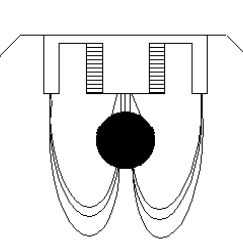
\includegraphics[width=0.3\textwidth]{./img/object_in_magnetic_field.png}
    \caption{Representation of the object in the magnetic field.}
    \label{fig:object_in_magnetic_field}
\end{figure}

By substituting the kinetic, potential, and dissipated energy terms into the Lagrange's equation, we can derive the equations of motion of the system.

\begin{equation}
    \begin{cases}
        \dot{z} = v_z                                                                                                                                         \\
        \dot{v_z} = \frac{1}{m} \left( \frac{1}{2} a L_d e^{-az} i_1^2 - \frac{1}{2} a L_d e^{-a(d - z)} i_2^2 - \frac{1}{2} C_d A \rho \dot{z} + m g \right) \\
        \dot{i_1} = \frac{1}{L_0 + L_d e^{-az}} \left( a L_d e^{-az} \dot{z} i_1 - R_1 i_1 + V_1 \right)                                                      \\
        \dot{i_2} = \frac{1}{L_0 + L_d e^{-a(d - z)}} \left( -a L_d e^{-a(d - z)} \dot{z} i_2 - R_2 i_2 + V_2 \right)                                         \\
        \dot{T_1} = \text{To be worked out}                                                                                                                   \\
        \dot{T_2} = \text{To be worked out}
    \end{cases}
\end{equation}

Where $v_z$ is the velocity of the ball, $i_1$ and $i_2$ are the currents flowing through the coils, and $T_1$ and $T_2$ are the temperatures of the coils.

The equations of motion of the system are highly non-linear and coupled, making the system hard to control.
